
\documentclass[12pt,epsfig,color,russian]{article}
\usepackage[russian]{babel}
\usepackage{epsfig}
\usepackage{color}

\topmargin=0cm
\hoffset -30mm
\voffset -12mm
\setlength{\unitlength}{1mm}
\parindent=10mm
\textheight=250mm
\textwidth=185mm
\pagestyle{empty}

\begin{document}
\sf\Large
\centerline{\LARGE\bf КОЛЕБАНИЯ и ВОЛНЫ}\vspace*{5mm}
\centerline{\underline{\Large\bf ГАРМОНИЧЕСКИЕ КОЛЕБАНИЯ}}

\noindent
\begin{picture}(185,65)(0,0)
 %\put(0,0){\framebox(185,65)[b]{}}
 \put(130,0){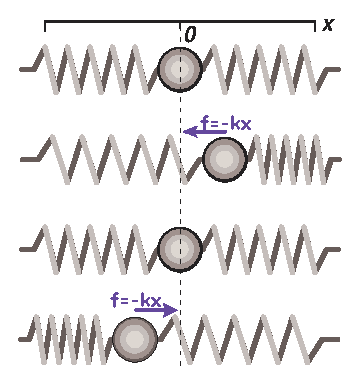
\includegraphics{GP014F01.eps}}
 \put(0,60){\makebox(0,0)[tl]{\parbox{125mm}{
Сила $f$, действующая на шарик с массой $m$, пропорциональна величине отклонения $x$ от точки равновесия 0 и направлена к этой точке: \fbox{$f=-kx$}. Такие силы называются {\bf упругими}. Под ее действием шарик возвращается. В момент прохода через 0 сила тоже =0, но из-за инерции шарик каждый раз проскакивает эту точку. Потенциальная энергия пружины переходит в кинетическую энергию шара and vice versa.
}}}
 \end{picture}\\

Другой пример (не самый лучший): маятник.\\
\begin{picture}(185,50)(0,0)
 %\put(0,0){\framebox(185,50)[b]{}}
 \put(155,0){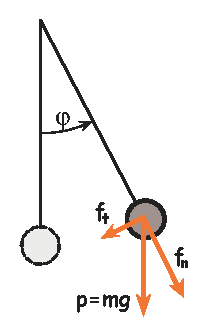
\includegraphics{GP014F02.eps}}
 \put(0,48){\makebox(0,0)[tl]{\parbox{145mm}{
Сила действует всегда только одна -- вес шарика $p=mg$, но при отклонении от вертикали на угол $\varphi$ меняется разложение веса на радиальную силу натяжения ($f_n=p\,\cos\varphi$) и тангенциальную силу возврата ($f_t=p\,\sin\varphi$).
Эта сила $f_t$ пропорциональна не углу отклонения $\varphi$, а его синусу. Но при небольших углах $\sin\varphi\simeq\varphi$, и тогда можно считать эту силу {\bf квазиупругой}.
}}}
 \end{picture}\\

В обоих перечисленных случаях возвращающая сила пропорциональна (или почти пропорциональна) отклонению. Это значит (по 2ЗН), что и ускорение пропорционально отклонению. В 1 случае мы получаем дифф.ур.:\vspace{-3mm}
\begin{equation}
m\,\ddot{x}=-k\,x
\end{equation}
Во втором случае вместо возвращающей силы $f_t$ лучше рассматривать ее момент $\mathcal{M}=f_t\times L$, где $L$ -- длина подвеса, а вместо массы маятника $m$ -- его момент инерции $\mathcal{I}=mL^2$. Используя вместо 2ЗН его аналог $\mathcal{M=I}\,\ddot{\varphi}$, получим для углового ускорения $mL^2\ddot{\varphi}=-mg\varphi$, или после сокращений:\vspace{-5mm}
\begin{equation}
L\,\ddot{\varphi}=-g\,\varphi
\end{equation}
у нас получились очень похожие уравнения. В обоих случаях множитель при ускорении (как линейном, так и угловом) характеризует инерционность подвижного элемента, а множитель при отклонении -- жесткость, то есть, масштаб возвращающей силы. Если переписать оба уравнения в виде
\begin{displaymath}
\ddot{x}=-\omega^2x
\end{displaymath}
где под $\omega^2$ понимать отношение $k/m$ в первом случае и $g/L$ во втором, то наиболее общее решение уравнения будет иметь вид:
\begin{equation}
x=A\,e^{i(\omega t+\alpha)},
\end{equation}
 причем аргументы $A$, $\omega$ и $\alpha$ находятся из каких-то дополнительных (на\-чаль\-ных или граничных) условий. Проверка:
\begin{displaymath}
\dot{x}=A\,e^{i(\omega t+\alpha)}\cdot i\omega;\hspace{10mm}\ddot{x}=
A\,e^{i(\omega t+\alpha)}\cdot (i\omega)^2=(-\omega^2)\cdot A\,e^{i(\omega t+\alpha)}
=-\omega^2x
\end{displaymath}
\begin{picture}(185,65)(0,0)
 %\put(0,0){\framebox(185,65)[b]{}}
 \put(120,0){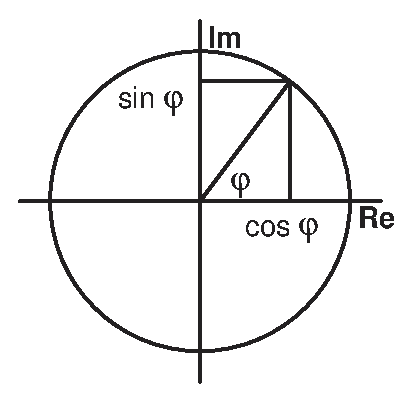
\includegraphics{GP014F03.eps}}
 \put(0,65){\makebox(0,0)[tl]{\parbox{120mm}{
\underline{Лирическое отступление}. Формула Эйлера \\
(Leonhard Euler, 1707 Basel -- 1783 СПб):
\begin{displaymath}
\begin{array}{rl}
e^x=&1+x+\frac{x^2}{2!}+\frac{x^3}{3!}+\frac{x^4}{4!}+\frac{x^5}{5!}+\frac{x^6}{6!}+\ldots\\
\rule{0mm}{9mm}\sin x=&x-\frac{x^3}{3!}+\frac{x^5}{5!}-\frac{x^5}{5!}+\ldots\\
\rule{0mm}{9mm}\cos x=&1-\frac{x^2}{2!}+\frac{x^4}{4!}-\frac{x^6}{6!}+\ldots\\
\rule{0mm}{9mm}e^{ix}=&\cos x +i\,\sin x
\end{array}
\end{displaymath}
}}}
 \end{picture}\\
Известно, что если $f_1(x)$ и $f_2(x)$ являются решениями дифференциального уравнения, то и их суперпозиция $a_1f_1(x)+a_2f_2(x)$ также является ре\-ше\-ни\-ем (\& vice versa).
Таким образом, в качестве уравнения гармонического ко\-ле\-ба\-ния можно использовать любое из трех:
\begin{eqnarray}
 x=&A\,e^{i(\omega t+\alpha)}\rule{12mm}{0mm} \label{Eq.exp} \\
 x=&A\,\sin (\omega t+\alpha) \label{Eq.sin} \\
 x=&A\,\cos (\omega t+\alpha) \label{Eq.cos}
\end{eqnarray}
Первое из них удобнее применять при работе с электрическими цепями, а последние два -- в механике, причем они более наглядны и отличаются друг от друга только фазой. Будем в дальнейшем пользоваться только одним из них (например, последним).

Итак, движение шарика на пружинке описывается уравнением
\begin{displaymath}
x=A\,cos(\omega t+\alpha)\hspace{10mm}\texttt{где}\;\;\omega^2=k/m
\end{displaymath}
а движение маятника (при небольшом его размахе) -- уравнением
\begin{displaymath}
\varphi=A\,cos(\omega t+\alpha)\hspace{10mm}\texttt{где}\;\;\omega^2=g/L
\end{displaymath}
В обоих случаях $A$ -- амплитуда колебания, т.е. его максимальное отклонение от точки равновесия, $(\omega t+\alpha)$ -- фаза, $\alpha$ -- начальная фаза,\\
\begin{picture}(185,50)(0,0)
 %\put(0,0){\framebox(185,60)[b]{}}
 \put(0,-5){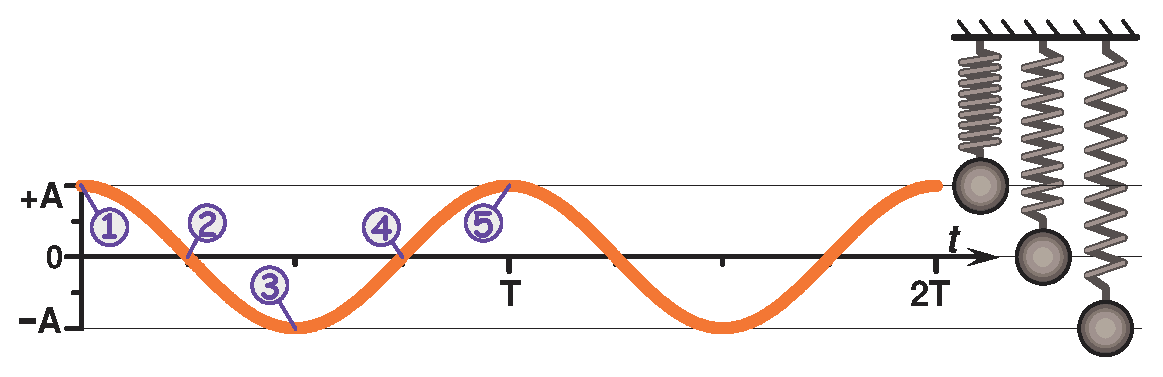
\includegraphics{GP014F04.eps}}
 \put(0,47){\makebox(0,0)[tl]{\parbox{150mm}{
 а $\omega$ -- частота. Для упрощения будем считать $\alpha$=0 и начнем рассмотрение с максимального отклонения. }}}
\end{picture}
\begin{enumerate}
\item ($\omega t$=0). В этот момент $\cos0$=1, отклонение максимально: $x$=+$A$, скорость $\vec{v}$=$\dot{x}$=--$\omega A\sin0$=0, и система покоится.
\item ($\omega t$=$\frac\pi2$). На этой фазе $\cos\frac\pi2$=0, шарик находится в положении рав\-но\-ве\-сия: $x$=0, но скорость $\vec{v}$=$\dot{x}$=--$\omega A\sin\frac\pi2$=--$\omega A$ максимальна, и шарик это положение по инерции проскакивает.
\item ($\omega t$=$\pi$). Теперь $\cos\pi$=--1, отклонение снова максимально, но с другим знаком: $x$=--$A$, скорость $\vec{v}$=$\dot{x}$=--$\omega A\sin\pi$=0, и шарик останавливается.
\item ($\omega t$=$\frac{3\pi}2$). На фазе $\cos\frac{3\pi}2$=0 шарик опять проходит положение равновесия ($x$=0) с максимальнй скоростью $\vec{v}$=$\dot{x}$=--$\omega A\sin\frac{3\pi}2$=+$\omega A$.
\item ($\omega t$=2$\pi$). Система вернулась в исходное состояние. Время, которое для этого потребовалось, --- {\bf период}: $T=\frac{2\pi}\omega$. Величина, обратная периоду --- {\bf частота} $\nu\equiv\frac1T$ (не путать с параметром $\omega$, который в 2$\pi$ раз больше и называется циклической частотой; циклическая частота показывает, не {\sl сколько колебаний} происходит в единицу времени, а на {\sl какой угол} в эту единицу времени меняется {\sl фаза} колебания).
\end{enumerate}
Уравнение гармонического колебания (\ref{Eq.cos}) может быть записано c помощью разных параметров:\vspace{-5mm}
\begin{equation}
x=A\,\cos(\omega t+\alpha)=A\,\cos(2\pi \nu t+\alpha)=A\,\cos(2\pi \frac t T+\alpha)
\end{equation}
Гармоническое движение -- бесконечно. Оно не уменьшается и не увели\-чи\-ва\-ет\-ся, происходит с постоянной частотой. При этом для конкретной колебательной системы {\bf частота не зависит от амплитуды}, с которой оно происходит, а зависит исключительно от динамических характеристик: для шарика на пружине -- это масса и жесткость; для маятника -- длина подвеса и напряженность гравитационного поля; для электрического ре\-зо\-нансного контура -- индуктивность и емкость; и т. п.
%Пример: период маятника длиной 24.5 см равен $T=2\pi\sqrt{L/g}\simeq1$ c.

Если какое-то из перечисленных свойств отсутствует --- то это НЕ {\bf гармоническое} колебание. Примеры таких негармонических колебаний:\\
\begin{picture}(185,90)(0,0)
 %\put(0,0){\framebox(185,90)[b]{}}
 \put(5,0){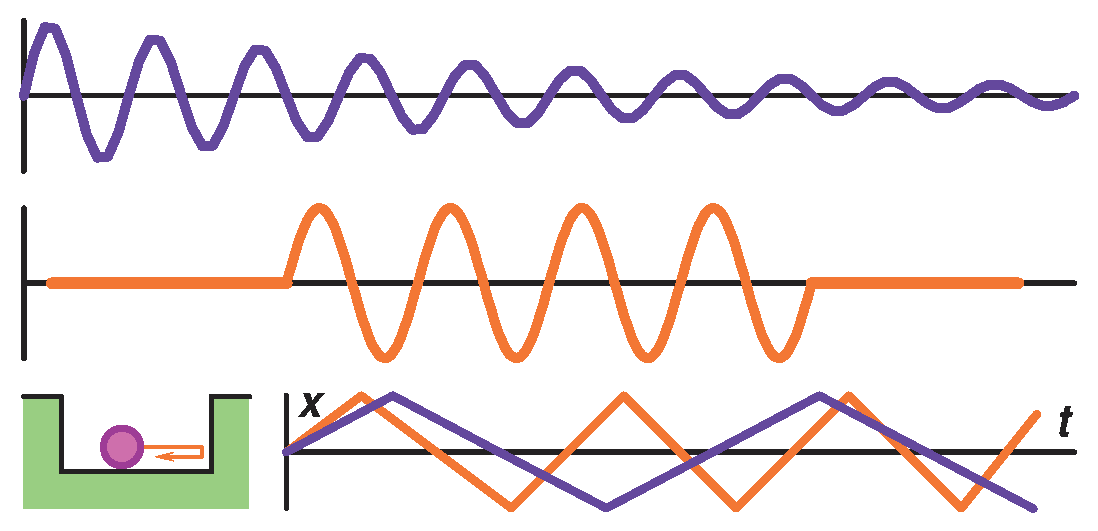
\includegraphics{GP014F05.eps}}
 \put(0,47){\makebox(0,0)[tl]{\parbox{150mm}{
 }}}
\end{picture}

В действительности, конечно, {\bf истинно гармонических} колебаний не бывает -- все они когда-то начинаются и когда-то заканчиваются, либо плавно затухают, либо частота их меняется со временем и зависит от амплитуды (т.е., это {\sl ``не совсем синус''}).

Тем не менее, гармонический осциллятор -- очень хорошее приближение к многим явлениям в природе. Свет, звук, строение атома и атомного ядра, -- все это может быть объяснено гармоническими колебаниями. Высокая стабильность г.к. $\Rightarrow$ часы; эталон частоты $\Rightarrow$ эталон длины.

Поговорим о \underline{\bf скорости}, \underline{\bf ускорении} и \underline{\bf энергии} в процессе гар\-мо\-ни\-че\-с\-ко\-го колебания.
\begin{displaymath}\begin{array}{rcl}
\texttt{\color{red}Смещение: }&x=&A\,\cos(\omega t+\alpha)\\
\texttt{\color{blue}Скорость: }&v=&\dot{x}=-\omega\,A\,\sin(\omega t+\alpha)
=\omega\,A\,\cos(\omega t+\alpha+\frac\pi2)\\
\texttt{\color{green}Ускорение: }&w=&\ddot{x}=-\omega^2\,A\,\cos(\omega t+\alpha)
=\omega^2\,A\,\cos(\omega t+\alpha+\pi)
\end{array}\end{displaymath}
\begin{picture}(185,50)(0,0)
 %\put(0,0){\framebox(185,60)[b]{}}
 \put(10,0){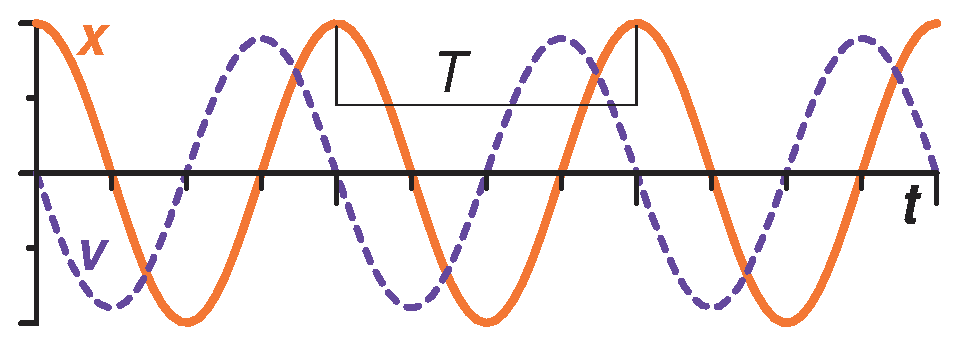
\includegraphics{GP014F06.eps}}
 \put(0,47){\makebox(0,0)[tl]{\parbox{150mm}{
 }}}
\end{picture}\\
Скорость описывается точно таким же законом ({\sl sin} или {\sl cos}), как и от\-кло\-не\-ние, но опережает его по фазе на $\frac\pi2$ (на четверть периода).

То же справедливо и для ускорения, но там опережение еще больше -- на $\pi$ (половину периода):\\
\begin{picture}(185,60)(0,0)
 %\put(0,0){\framebox(185,60)[b]{}}
 \put(10,0){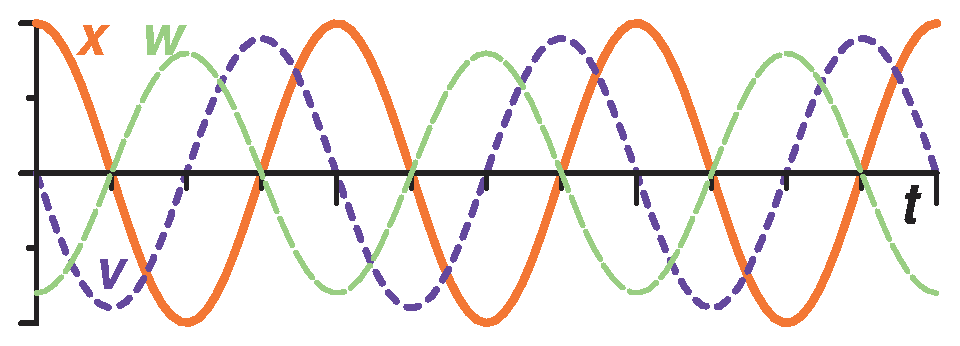
\includegraphics{GP014F07.eps}}
 \put(0,47){\makebox(0,0)[tl]{\parbox{150mm}{
 }}}
\end{picture}\\
Таким образом, скорость (и, соответственно, кинетическая энергия) до\-сти\-га\-ет своего максимума при прохождении точек равновесия.

Ускорение же вызывается действием возвращающей силы, а она (сила) пропорциональна отклонению и, следовательно, ускорение максимально при мак\-си\-маль\-ном отклонении, но направлено в противоположную сторону.

Кинетическая энергия в любой момент (с учетом того, что $\omega^2=k/m$):
\begin{displaymath}
E_k=\frac12mv^2=\frac12mA^2\omega^2\sin^2(\omega t+\alpha)
=\frac12kA^2\sin^2(\omega t+\alpha)
\end{displaymath}

Если шарик колеблется на пружине \underline{горизонтально} (это для упрощения; результат будет тот же), то потенциальная энергия равна\vspace{-3mm}
\begin{displaymath}
E_p=\frac12kx^2=\frac12kA^2\cos^2(\omega t+\alpha)
\end{displaymath}
Полная энергия системы (сумма $E_k+E_p$) составит\vspace{-3mm}
\begin{displaymath}
E=E_k+E_p=\frac12kA^2\sin^2(\omega t+\alpha)+\frac12kA^2\cos^2(\omega t+\alpha)=
\frac12kA^2
\end{displaymath}
\begin{picture}(185,50)(0,0)
 %\put(0,0){\framebox(185,60)[b]{}}
 \put(10,0){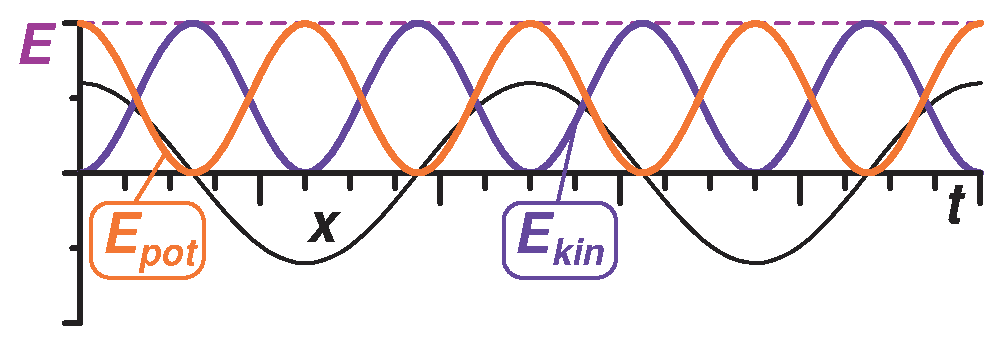
\includegraphics{GP014F08.eps}}
 \put(0,47){\makebox(0,0)[tl]{\parbox{150mm}{
 }}}
\end{picture}\\
Как видим, кинетическая и потенциальная энергия при колебании переходят друг в друга с частотой, в 2 раза большей (потому как $E_p(-x)=E_p(+x)$, а $E_k(-v)=E_k(+v)$), в то время как их сумма остается постоянной, пропорциональной жесткости и квадрату амплитуды.\\
\begin{picture}(185,50)(0,0)
 %\put(0,0){\framebox(185,50)[b]{}}
 \put(133,0){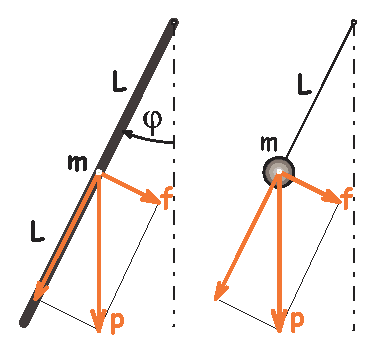
\includegraphics{GP014F10.eps}}
 \put(0,45){\makebox(0,0)[tl]{Рассмотрим для примера два маятника с массой $m$ -- }}
 \put(0,37){\makebox(0,0)[tl]{физический (стержень длиной $2L$) и математический}}
 \put(0,29){\makebox(0,0)[tl]{(материальную точку на невесомом подвесе $L$).}}
 \put(0,21){\makebox(0,0)[tl]{\parbox{130mm}{
   Центры масс обоих маятников лежит на одинаковом расстоянии $L$ от точки подвеса. Возвращающий момент силы тоже одинаков:
 }}}
\end{picture}\vspace*{-3mm}
  \begin{displaymath}
  \mathcal{M}=pL\sin\varphi\simeq pL\varphi;\hspace{10mm}
  \texttt{или с учетом направления: }\;\;
  \vec{\mathcal{M}}\simeq-pL\vec{\varphi}\vspace{-3mm}
  \end{displaymath}
Различие появляется, когда мы начинаем вычислять угловое ускорение: $\ddot{\varphi}=\mathcal{M}/\mathcal{I}$. Дело в том, что моменты инерции $\mathcal{I}_1$ и $\mathcal{I}_2$ у маятников разные:\vspace{-3mm}
  \begin{displaymath}
  \texttt{для стержня: }\;\; \mathcal{I}_1=mL^2+\frac{mL^2}3=\frac43mL^2\hspace{10mm}
  \texttt{для точки:   }\;\; \mathcal{I}_2=mL^2\vspace{-1mm}
  \end{displaymath}
Поэтому и периоды колебаний $T=2\pi\sqrt{\mathcal{I}/mgL}$ тоже будут отличаться: \vspace{-1mm}
  \begin{displaymath}
  T_2=2\pi\sqrt{\frac{L}{g}}\hspace{20mm}T_1=2\pi\sqrt{\frac{4L}{3g}}\simeq1.15\;T_2
  \end{displaymath}

\underline{\bf Сложение колебаний}\\
\begin{picture}(185,55)(0,0)
 %\put(0,0){\framebox(185,55)[b]{}}
 \put(120,0){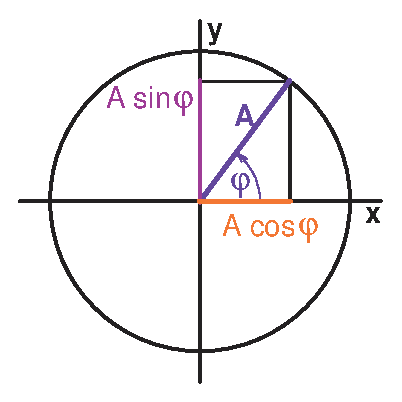
\includegraphics{GP014F11.eps}}
 \put(0,52){\makebox(0,0)[tl]{\parbox{115mm}{
Любое гармоническое колебание, записанное в виде $x_1=A\,\cos(\omega t+\alpha_1)$, можно формально представить как проекцию на ось $\vec{x}$ от вра\-ща\-ю\-щегося с частотой $\omega$ вектора, длина которого равна амплитуде $A$. Тогда, если в одном и том же направлении происходят од\-но\-вре\-мен\-но 2 колебания с одинаковой частотой:
 }}}
\end{picture}\\
$x_1=A\,\cos(\omega t+\alpha_1)$ и $x_2=B\,\cos(\omega t+\alpha_2)$ -- то суммарное движение, равное суперпозиции двух гармоничеких осцилляций, представляет собой \begin{picture}(185,65)(0,0)
 %\put(0,0){\framebox(185,65)[b]{}}
 \put(0,0){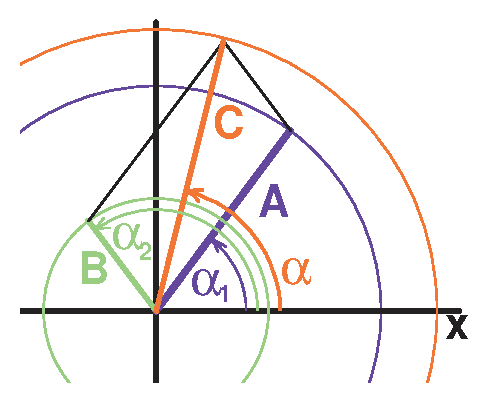
\includegraphics{GP014F12.eps}}
 \put(80,62){\makebox(0,0)[tl]{\parbox{105mm}{
проекцию вектора, равного сумме двух амплитуд (так как частоты одинаковы, то оба вектора вращаются синхронно, и угол между ними постоянен $\Rightarrow$ суммарный вектор тоже постоянен по длине).
  \begin{displaymath}
x=x_1+x_2=C\,\cos(\omega t+\alpha)
  \end{displaymath}
  \begin{displaymath}
C^2=A^2+B^2+2AB\cos(\alpha_2-\alpha_1)
  \end{displaymath}
   }}}
\end{picture}\\
И это будет тоже гармоническое колебание!\\
\begin{picture}(185,30)(0,0)
 %\put(0,0){\framebox(185,40)[b]{}}
 \put(10,0){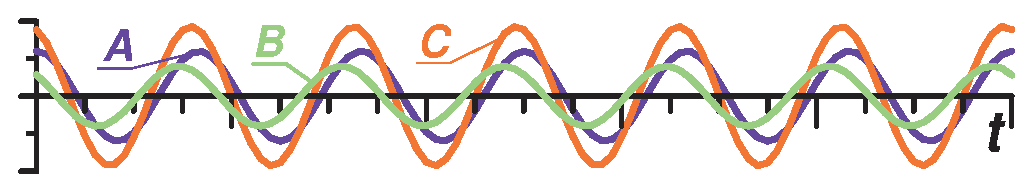
\includegraphics{GP014F13.eps}}
\end{picture}\\
Другая картина при сложении колебаний с РАЗНОЙ частотой. Здесь угол между складываемыми векторами все время меняется $\Rightarrow$ суммарный век\-тор $\neq$ const., и получается уже НЕ гармоническое колебание.\\
\begin{picture}(185,40)(0,0)
 %\put(0,0){\framebox(185,40)[b]{}}
 \put(10,0){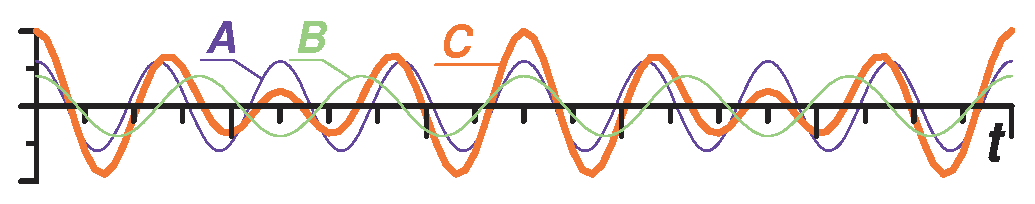
\includegraphics{GP014F14.eps}}
\end{picture}\\
В зависимости от того, как соотносятся частоты складываемых колебаний, получаются совершенно разные (но очень важные!) результаты. Рас\-смо\-т\-рим их подробнее.
\begin{itemize}
\item {\bf Частоты отличаются очень мало.} Пусть $\omega_2=\omega_1+2\varepsilon$, а амплитуды обоих колебаний равны друг другу: $A=B$. Длина суммарного вектора $\vec{C}$ (по теореме косинусов) зависит от разности фаз колебаний:
    \begin{displaymath}
    C^2=A^2+B^2+2AB\cos(\omega_2-\omega_1)t=
    2A^2\cdot\left(1+\cos2\varepsilon t\right)=
    4A^2\cos^2\varepsilon t
    \end{displaymath}
    \begin{displaymath}
    C=\sqrt{4A^2\cos^2\varepsilon t}=2A\cos\varepsilon t
    \end{displaymath}

    Получилось, что длина результирующего вектора будет меняться со временем как $\cos\varepsilon t$, то есть, возникает что-то вроде БИЕНИЙ с этой разностной частотой\\
    \begin{picture}(185,30)(0,0)
     %\put(0,0){\framebox(185,40)[b]{}}
      \put(0,0){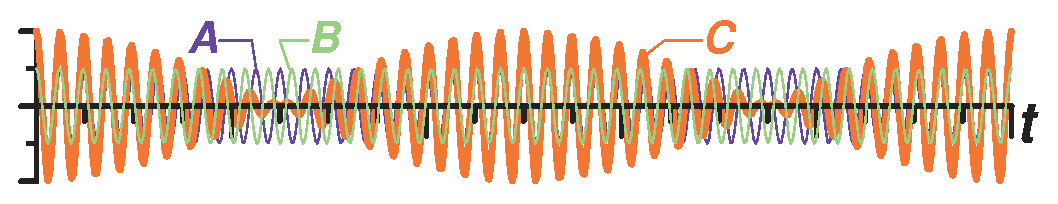
\includegraphics{GP014F15.eps}}
    \end{picture}\\
    Фаза этого суммарного вектора $\vec{C}$ равна среднему арифметическому от фаз слагаемых векторов, поэтому его проекция будет
    \begin{displaymath}
     x=C\,\cos\left(\frac{\omega_1+\omega_2}2t+\alpha\right)=
     \left(2A\cos\varepsilon t\right)\cdot\cos\left(\frac{\omega_1+\omega_2}2t+\alpha\right)
    \end{displaymath}
    \hspace{10mm}То есть, получилось как бы гармоническое колебание с частотой $\omega=(\omega_1+\omega_2)/2$, амплитуда которого не постоянна, но медленно меняется с частотой $\varepsilon=(\omega_2-\omega_1)/2$.\\
    \hspace{10mm}Это явление широко используется в радиотехнике для преобразования слишком высокой принимаемой несущей частоты $f_s$ в удобную про\-ме\-жу\-точную частоту $f_0$. Для этого регулируемый генератор ({\bf гетеродин})\\
    \begin{picture}(185,45)(0,0)
     %\put(0,0){\framebox(185,50)[b]{}}
      \put(55,0){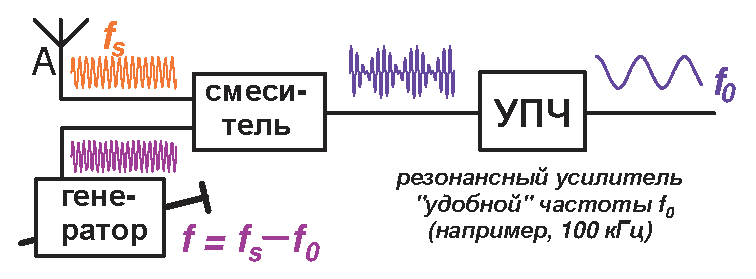
\includegraphics{GP014F16.eps}}
      \put(0,42){\makebox(0,0)[tl]{\parbox{53mm}{
     производит свою до\-пол\-ни\-тель\-ную ча\-с\-то\-ту $f$, ко\-то\-рая под\-би\-ра\-ет\-ся так, чтобы $f_0$=$f_s$--$f$.
    }}}
    \end{picture}
\item {\bf Частоты отличаются в целое число раз.} Пусть $\omega_2=2\omega_1$, сдвиг фаз $\varphi=\pi/2$ и 0, а отношение амплитуд $A_2/A_1$=0.5. Построив с помощью компьютера такие графики, а также графики с добавкой $\omega_3=3\omega_1$ и $\omega_4=4\omega_1$, получим:\\
    \begin{picture}(185,220)(0,0)
     %\put(0,0){\framebox(185,220)[b]{}}
      \put(0,165){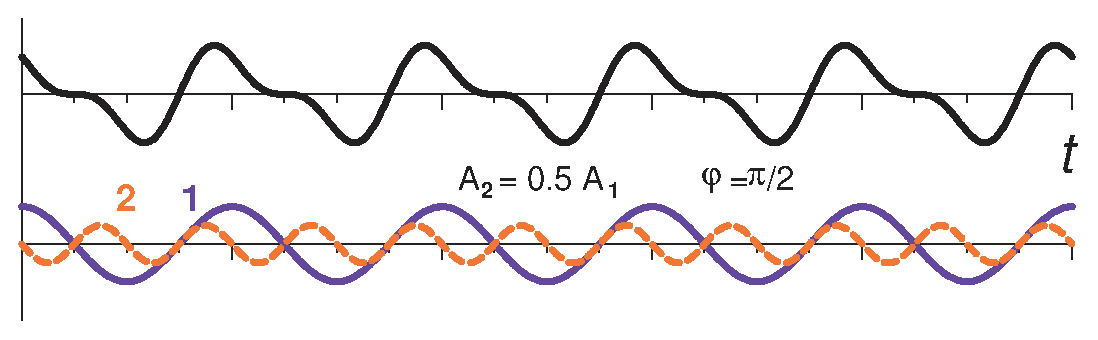
\includegraphics{GP014F19.eps}}
      \put(0,110){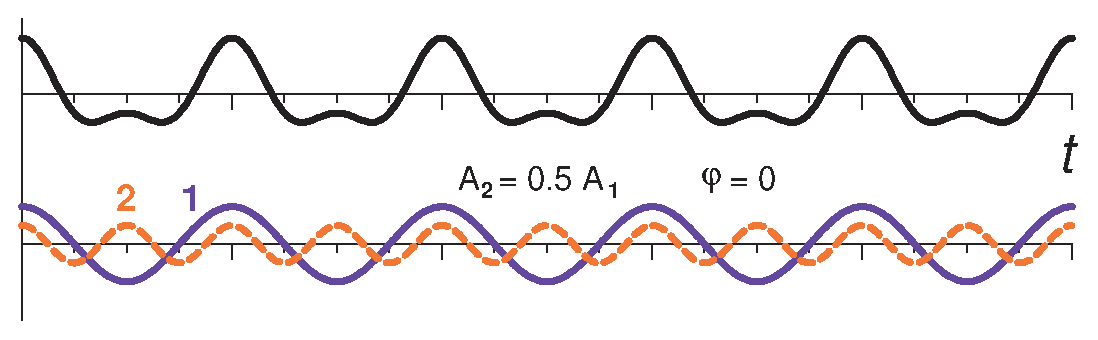
\includegraphics{GP014F17.eps}}
      \put(0, 55){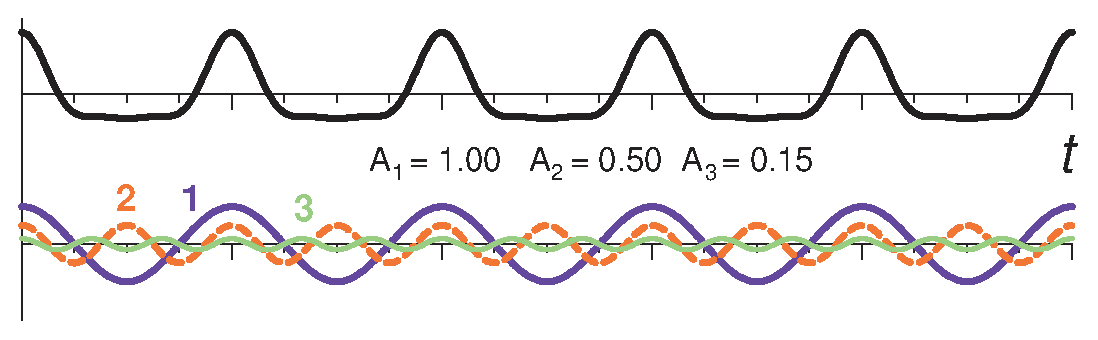
\includegraphics{GP014F21.eps}}
      \put(0,  0){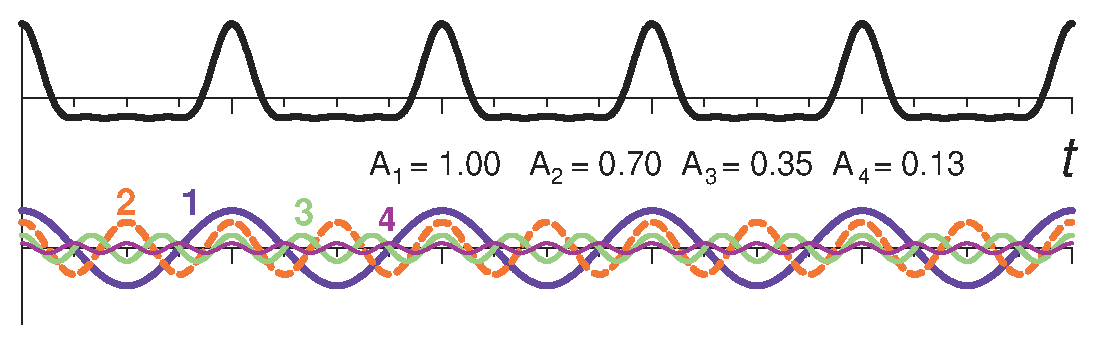
\includegraphics{GP014F22.eps}}
    \end{picture}\\
    Видим, что, комбинируя амплитуды и фазы кратных частот ({\bf высших гармоник}), можно получить любую форму функции с периодом, соответствующим основной частоте $\omega_1$.\\
    На этом основан анализ Фурье -- разложение произвольной пе\-ри\-о\-ди\-чес\-кой функции $f(x)$ в ряд гармоник (или непериодической -- в непрерывный частотный спектр).\\
    Jean Baptiste Joseph Fourier (1768--1830, Paris, FR)\\
    \begin{displaymath}
     f(x)=\frac{A_0}2+\sum\limits_{n=1}^{\infty}\left(A_n\,\cos (nx)+B_n\,\sin (nx)\right)
    \end{displaymath}
    где амплитуды $A_n$ и $B_n$ находятся из формул
    \begin{displaymath}
     A_n=\frac1\pi \int\limits_{-\pi}^{+\pi}f(x)\cos(nx)\,dx
    \end{displaymath}
    \begin{displaymath}
     B_n=\frac1\pi \int\limits_{-\pi}^{+\pi}f(x)\sin(nx)\,dx
    \end{displaymath}
    \vspace{5mm}
    Пример: разложить в ряд Фурье симметричный меандр:\\
    \begin{picture}(185,40)(0,0)
      %\put(0,0){\framebox(185,40)[b]{}}
      \put(0,0){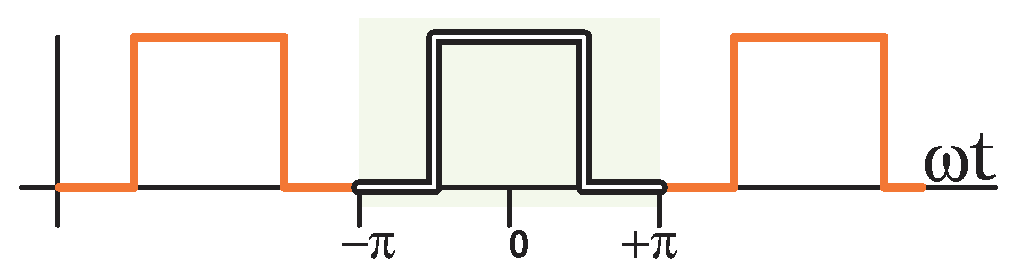
\includegraphics{GP014F27.eps}}
    \end{picture}\\
    Решение: Рассмотрим отрезок длиной в один период, расположив его симметрично относительно начала шкалы. Тогда $f(x)$=1 при $\-pi/2<x<+\pi/2$ и $f(x)$=0
    правее и левее. Вычисляем амплитуды $A_n$ и $B_n$ для $n=0,1,2,3...$.
    Сначала заметим, что наша функция $f(x)$ -- четная (то есть, $f(x)$=$f(-x)$). Из этого следует, что синусы в разложении участвовать не должны, и все коэф-ты $B_n=0$. Проверим это для произвольного $n$:
    \begin{displaymath}
    \pi\cdot B_n=\int\limits_{-\pi/2}^{+\pi/2}\sin(nx)\,dx
     =\int\limits_{-n\pi/2}^{+n\pi/2}\sin(z)\,\frac{dz}n
     =\left.-\frac{\cos(z)}{n}\right|_{-n\pi/2}^{+n\pi/2}=0
    \end{displaymath}
    Последнее равенство обусловлено тем, что $\forall\varphi$ всегда $\cos(\varphi)\equiv\cos(-\varphi)$. Теперь посчитаем коэффициенты при косинусах. $A_0$ -- это особый случай:
    \begin{displaymath}
    \pi\cdot A_0=\int\limits_{-\pi/2}^{+\pi/2}1\,\cos(0)\,dx
     =\left.x\right|_{-\pi/2}^{+\pi/2}=\pi\;\;\;\;\Rightarrow\;A_0=1.0
    \end{displaymath}
    Остальные $A_n$ находим заменой переменной интегрирования $nx\rightarrow z$:
    \begin{displaymath}
    \pi\cdot A_n=\int\limits_{-\pi/2}^{+\pi/2}\cos(nx)\,dx
     =\int\limits_{-n\pi/2}^{+n\pi/2}\cos(z)\,\frac{dz}n
     =\left.\frac{\sin(z)}{n}\right|_{-n\pi/2}^{+n\pi/2}=\frac2n\sin\frac{n\pi}2
    \end{displaymath}
    Для четных $n=2k$ полученная величина $\sin\frac{n\pi}2=\sin(k\pi)=0$, а для нечетных эта величина поочередно равна или +1, или --1.

    Таким образом, получаем: $B_n$=0; $A_0=1.0$; $A_1=+\frac2\pi$; $A_3=-\frac2{3\pi}$; $A_5=+\frac2{5\pi}$; $A_7=-\frac2{7\pi}$; $A_9=+\frac2{9\pi}$; $A_{11}=-\frac2{11\pi}$; $A_{13}=+\frac2{13\pi}$;\rule{0mm}{8mm} ...\\
    \begin{picture}(185,140)(0,0)
      %\put(0,0){\framebox(185,140)[b]{}}
      \put(10,0){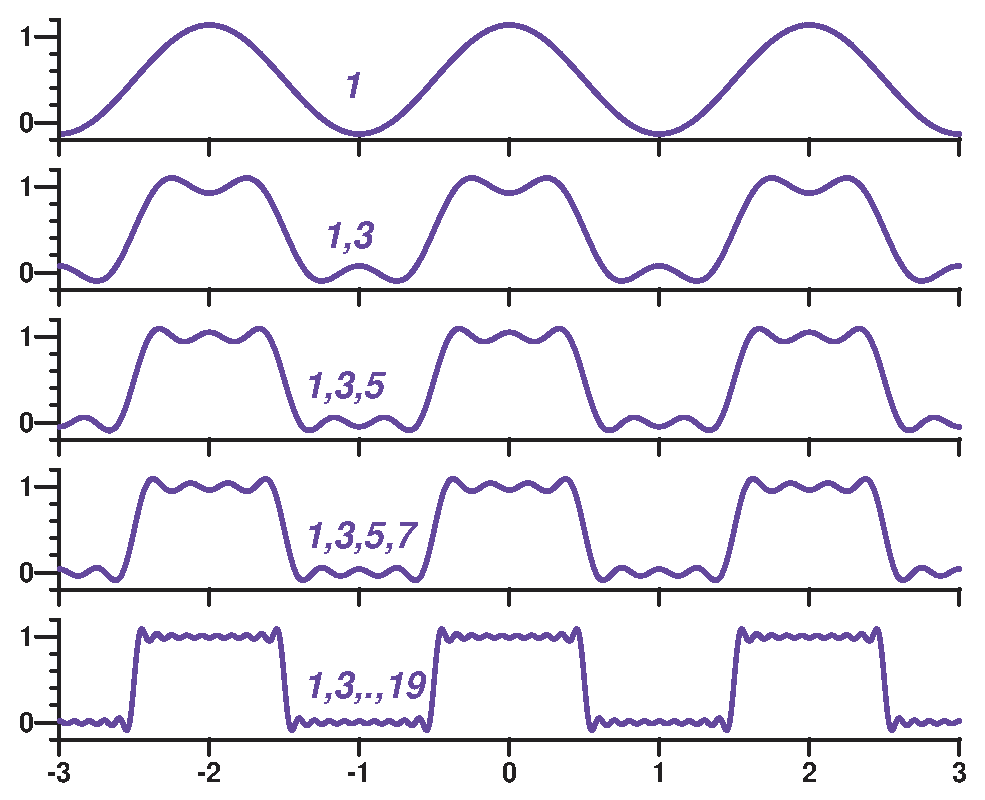
\includegraphics{GP014F28.eps}}
    \end{picture}\\
    \begin{picture}(185,40)(0,0)
      %\put(0,0){\framebox(185,40)[b]{}}
      \put(10,0){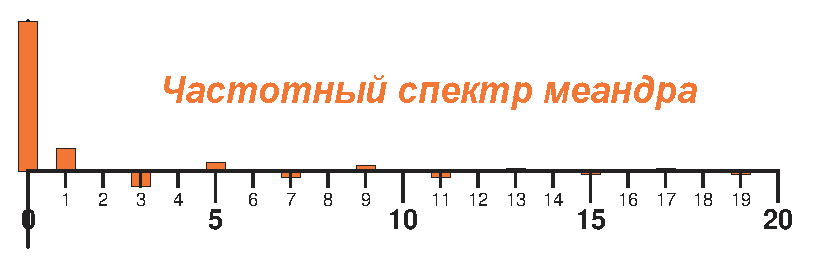
\includegraphics{GP014F30.eps}}
    \end{picture}\\
    \end{itemize}
\underline{\bf Сложение колебаний вдоль разных осей}\\
Пусть для начала это перпендикулярные оси $\vec{x}$ и $\vec{y}$, и частоты равны. Тогда
\begin{displaymath}
\left\{
\begin{array}{lcr}
x&=&A_1\,\cos(\omega t+\alpha_1)\\
y&=&A_2\,\cos(\omega t+\alpha_2)
\end{array}
\right.
\end{displaymath}
Чтобы отследить траекторию, исключим отсюда время $t$. Для этого пе\-ре\-пи\-шем уравнения, домножим их на $\cos(\alpha_{2,1})$ и вычтем:
\begin{displaymath}
\left\{
\begin{array}{lcr}
\frac{x}{A_1}&=&\cos(\omega t)\cdot\cos(\alpha_1)-\sin(\omega t)\cdot\sin(\alpha_1) \\
\frac{y}{A_2}&=&\cos(\omega t)\cdot\cos(\alpha_2)-\sin(\omega t)\cdot\sin(\alpha_2)
\end{array}
\right|
\begin{array}{l}
\cdot\cos(\alpha_2)\\
\cdot\cos(\alpha_1)
\end{array}
\end{displaymath}
\begin{displaymath}
\frac{x}{A_1}\cos(\alpha_2)-\frac{y}{A_2}\cos(\alpha_1)=
\sin(\omega t)\cdot\sin(\alpha_2-\alpha_1)
\end{displaymath}
Если теперь сделать то же самое, но домножать не на $\cos(\alpha_{2,1})$ а на $\sin(\alpha_{2,1})$, то получится
\begin{displaymath}
\frac{x}{A_1}\sin(\alpha_2)-\frac{y}{A_2}\sin(\alpha_1)=
\cos(\omega t)\cdot\sin(\alpha_2-\alpha_1)
\end{displaymath}
Если теперь возвести в квадрат и сложить оба полученных уравнения, то
 $\omega t$ уходит, и остается уравнение траектории:
\begin{displaymath}
\frac{x^2}{A_1^2}+\frac{y^2}{A_2^2}-\frac{2xy}{A_1A_2}\cos(\alpha_2-\alpha_1)=
\sin^2(\alpha_2-\alpha_1)
\end{displaymath}
Это -- уравнение ЭЛЛИПСА, характеристики которого зависят от разности фаз $\theta=(\alpha_2-\alpha_1)$.
\begin{itemize}
\item Пусть фазы совпадают: $\theta=0$, и $\alpha_2=\alpha_1=\alpha$. Тогда
\begin{displaymath}
\frac{x^2}{A_1^2}+\frac{y^2}{A_2^2}-\frac{2xy}{A_1A_2}=0
\hspace{10mm}\Rightarrow\hspace{10mm}
\left(\frac{x}{A_1}-\frac{y}{A_2}\right)^2=0
\hspace{10mm}\Rightarrow\hspace{10mm}
\frac xy=\frac{A_1}{A_2}
\end{displaymath}
Это -- прямая линия. Если колебания не {\sl в фазе}, а {\sl в противофазе} ($\theta=\pi$), то тоже будет прямая, но наклон -- в другую сторону:\\
    \begin{picture}(185,55)(0,0)
     %\put(0,0){\framebox(185,55)[b]{}}
      \put(0,0){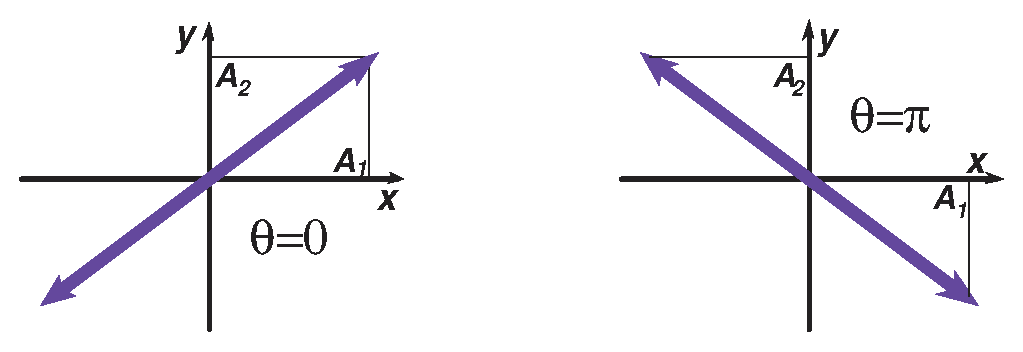
\includegraphics{GP014F23.eps}}
    \end{picture}\\
Колебание вдоль этой наклонной прямой будет тоже гармоническим с таким же периодом и с амплитудой $s=\sqrt{A_1^2+A_2^2}$.
\item Если фазы сдвинуты на $\pi/2$, то получается уравнение эллипса:
\begin{displaymath}
\hspace{60mm}\left(\frac{x}{A_1}\right)^2+\left(\frac{y}{A_2}\right)^2=1
\end{displaymath}
    \begin{picture}(185,55)(0,0)
     %\put(0,0){\framebox(185,55)[b]{}}
      \put(0,0){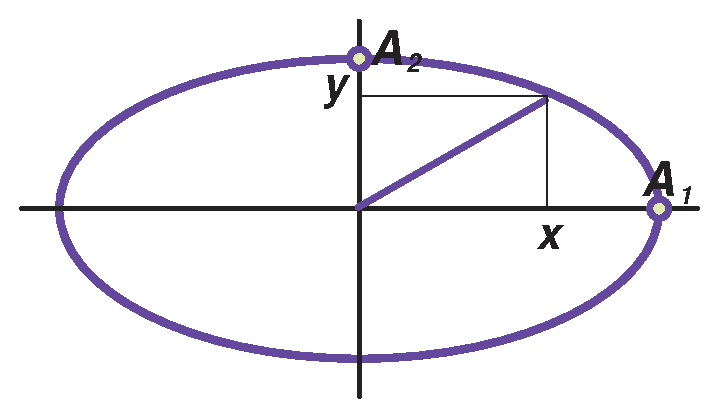
\includegraphics{GP014F24.eps}}
    \end{picture}\\
\item А вообще, при разном сдвиге фаз получаются разные эллипсы:\\
    \begin{picture}(185,30)(0,0)
      %\put(0,0){\framebox(185,30)[b]{}}
      \put(0,0){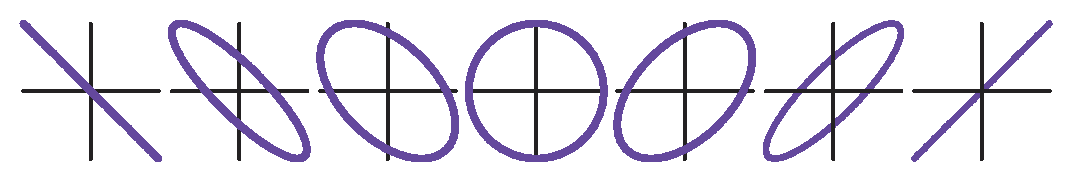
\includegraphics{GP014F25.eps}}
    \end{picture}\\
    Значит, движение точки по эллипсу можно представить как сумму двух гармонических взаимно $\perp$ колебаний.
\item Если частоты (или периоды) соотносятся как целые числа, то получаются не только эллипсы, но и более сложные фигуры Лисажу:\\
    \begin{picture}(185,30)(0,0)
      %\put(0,0){\framebox(185,30)[b]{}}
      \put(0,0){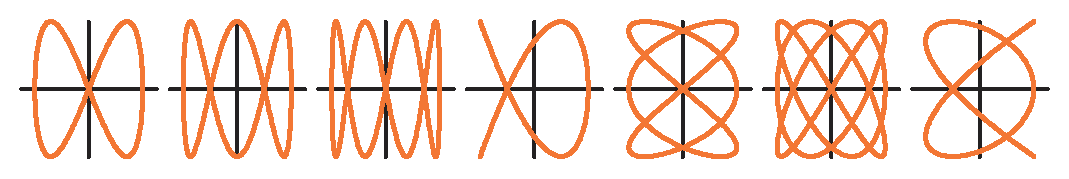
\includegraphics{GP014F26.eps}}
    \end{picture}\\
\end{itemize}\vspace{10mm}
\underline{\bf Затухающие колебания}\\
Любое реальное колебание без внешней подпитки рано или поздно затухает. Это вызвано потерей энергии на трение в подвесе, сопротивление внешней среды, нагрев из-за ненулевого электрического сопротивления, электро-магнитное излучение и т. п. Для примера рассмотрим колебание в вязкой среде (в воздухе). В этом случае сила трения пропорциональна скорости тела (в первом приближении!), и тогда уравнение по 2ЗН выглядит так:\vspace{-3mm}
\begin{displaymath}
m\ddot{x}=-kx-r\dot{x}\;\;\;\;\;\texttt{или}\;\;\;\;\;\ddot{x}=-\frac kmx-\frac rm\dot{x}\vspace{-3mm}
\end{displaymath}
Введем обозначения:\vspace{-5mm}
\begin{displaymath}
\frac km\equiv\omega_0^2;\;\;\;\;\frac rm\equiv2\beta
\end{displaymath}
Тогда дифф. ур. преобразуется в\vspace{-3mm}
\begin{displaymath}
\ddot{x}=-\omega_0^2x-2\beta\dot{x}\vspace{-3mm}
\end{displaymath}
Как его решать? Если бы не было торможения ($\beta\rightarrow0$), то все свелось бы к гармоническому осциллятору. Но это, к сожалению не так. Интуиция подсказывает, что с каждым очередным колебанием система должна терять примерно одну и ту же {\bf долю} своей энергии, $\Rightarrow$ амплитуда должна убывать со временем {\bf экспоненциально}, причем крутизна экспоненты должна быть пропорциональна коэффициенту сопротивления. Введем такую за\-ме\-ну переменной:\vspace{-3mm}
\begin{displaymath}
x=z\,e^{-\beta t},\;\;\;\;\;\;\;\dot{x}=\dot{z}\,e^{-\beta t}-\beta\,z\,e^{-\beta t},
\;\;\;\;\;\;\;\ddot{x}=\ddot{z}\,e^{-\beta t}-2\beta\,\dot{z}\,e^{-\beta t}+\beta^2\,z\,e^{-\beta t}
\end{displaymath}
Подставив это вместо $x$, $\dot{x}$ и $\ddot{x}$ в наше дифф. ур-ние, получим
\begin{displaymath}
\ddot{z}-2\beta\dot{z}+\beta^2z=-\omega_0^2z+2\beta^2z-2\beta\dot{z}\;\;\;\;\;\;\;\texttt{или}\;\;\;
\ddot{z}=-(\omega_0^2-\beta^2)\,z
\end{displaymath}
Это последнее уравнение -- в точности такое же, как и для гармонического колебания, только частота здесь несколько уменьшилась: $\omega^2\equiv(\omega_0^2-\beta^2)$. В качестве его решения получаем любое из следующих выражений:
\begin{displaymath}\begin{array}{rl}
x=&A_0\cdot e^{-\beta t}\cdot e^{i(\omega t+\alpha)}\\
x=&A_0\cdot e^{-\beta t}\cdot \sin\left(\omega t+\alpha\right)\\
x=&A_0\cdot e^{-\beta t}\cdot \cos\left(\omega t+\alpha\right)
\end{array}\end{displaymath}
причем не следует забывать, что здесь $\omega^2\equiv(\omega_0^2-\beta^2)$. Как видим, сопротивление играет двоякую роль: уменьшает амплитуду колебаний со временем (она теперь не постоянна) и уменьшает частоту (частота посто\-ян\-на, но меньше по величине).\\
    \begin{picture}(185,60)(0,0)
      %\put(0,0){\framebox(185,60)[b]{}}
      \put(10,0){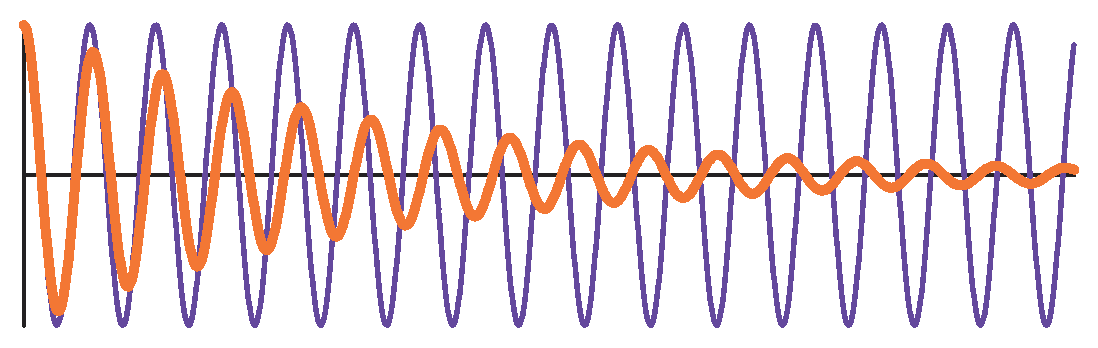
\includegraphics{GP014F29.eps}}
    \end{picture}\\
Либо можно сказать, что период колебаний в вязкой среде стал больше:\vspace{-3mm}
\begin{displaymath}
T=\frac{2\pi}{\sqrt{\omega_0^2-\beta^2}}>\frac{2\pi}{\omega_0}
\end{displaymath}
Если взять отношение амплитуд для двух соседних периодов -- то это будет константа, логарифм которой называется {\bf логарифмическим де\-к\-ре\-ме\-н\-том затухания} $\lambda$.\vspace{-6mm}
\begin{displaymath}
\lambda=\ln\frac{A_0\,e^{-\beta t}}{A_0\,e^{-\beta(t+T)}}=\ln\,e^{\beta T}=\beta T
\end{displaymath}
Тогда можно, во-первых, записать уравнение колебаний в новом виде:\vspace{-3mm}
\begin{displaymath}
x=A_0\cdot e^{-\lambda\frac tT}\cdot \cos\left(2\pi\frac tT+\alpha\right)
\end{displaymath}
и, во-вторых, определять коэф-т сопротивления среды $r$ из затухания колебаний:
\begin{displaymath}
r=2\beta m=2\frac{\lambda}Tm
\end{displaymath}
Пример: лог.декркмент $\lambda$=0.02; во сколько раз уменьшится амплитуда после 100 колебаний? \\
Решение: в начальный момент ($t$=0) амплитуда = $A_0$. В последующее время $t$ формула колебания выглядит как \vspace{-5mm}
\begin{displaymath}
\hspace{30mm}x=A_0\cdot e^{-\lambda\frac tT}\cdot \cos\left(2\pi\frac tT+\alpha\right)
\end{displaymath}
через 100 периодов ($t=100\,T$) амплитуда станет равна\vspace{-3mm}
\begin{displaymath}
A=A_0\cdot e^{-\lambda\frac tT}=A_0\cdot e^{-0.02\cdot100}=A_0\cdot e^{-2}\simeq0.135A_0\simeq\frac{A_0}{7.39}
\end{displaymath}

Если как-то компенсировать потери на трение, то есть, в нужные моменты подталкивать систему, то затухания не будет. \underline{\bf Автоколебания.} Пример: балансир часов. Находясь в нужной фазе, балансир с помощью храпового механизма на короткое время дает возможность пружине себя подтолкнуть. Другой пример: хлопанье флага на ветру.\\
    \begin{picture}(185,40)(0,0)
      %\put(0,0){\framebox(185,40)[b]{}}
      \put(10,0){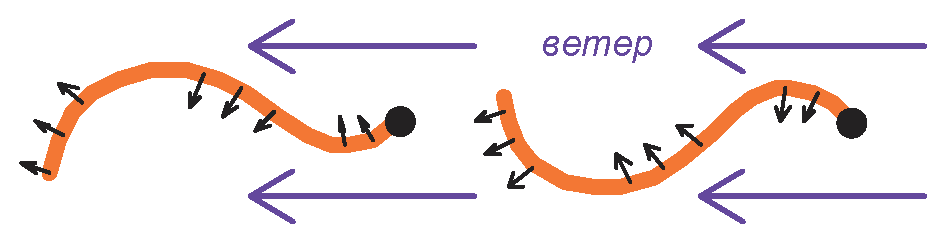
\includegraphics{GP014F35.eps}}
    \end{picture}\\



\underline{\bf Вынужденные колебания}\\
\begin{picture}(185,40)(0,0)
 %\put(0,0){\framebox(185,40)[b]{}}
 \put(170,0){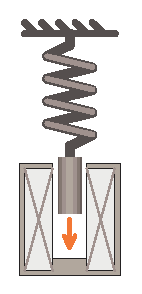
\includegraphics{GP014F31.eps}}
 \put(0,33){\makebox(0,0)[tl]{\parbox{165mm}{
 Что будет, если кроме упругой силы и сил сопротивления, на тело действует внешняя периодическая {\bf вынуждающая} сила? Например, эта сила меняется во времени как\vspace{-4mm}
\begin{displaymath}
 f(t)=H\,\cos(\omega t)\vspace{-3mm}
\end{displaymath}
Уравнение, выражающее 2ЗН будет следующим:
 }}}
\end{picture}\\
\begin{displaymath}\vspace{-3mm}
m\ddot{x}=-kx-r\dot{x}+H\cos(\omega t)\vspace{-3mm}
\end{displaymath}
Введя обозначения:\vspace{-5mm}
\begin{displaymath}
\frac km\equiv\omega_0^2;\;\;\;\;\frac rm\equiv2\beta;\;\;\;\;h\equiv\frac Hm
\end{displaymath}
получим такое дифф. уравнение\vspace{-3mm}
\begin{displaymath}
\ddot{x}=-\omega_0^2x-2\beta\dot{x}+h\cos(\omega t)\vspace{-3mm}
\end{displaymath}
Будем искать решение в виде $x=A\cos(\omega t +\alpha)$, то есть, по нашему мнению, внешняя сила должна ``победить''. Если это так, то первая и вторая производные равны, соответственно\vspace{-3mm}
\begin{displaymath}
\dot{x}=-A\omega\sin(\omega t +\alpha);\;\;\;\;\ddot{x}=-A\omega^2\cos(\omega t +\alpha)
\end{displaymath}
Подставив все это в исходное уравнение, получим:
\begin{displaymath}
-A\omega^2\cos(\omega t +\alpha)=-A\omega_0^2\cos(\omega t +\alpha)+2A\beta \omega\sin(\omega t +\alpha)+h\cos(\omega t)
\end{displaymath}
Приведем подобные члены:
\begin{displaymath}
A(\omega^2-\omega_0^2)\cos(\omega t +\alpha)+2A\beta\omega\sin(\omega t +\alpha)+h\cos(\omega t)=0
\end{displaymath}
 и заменим sin и cos суммы углов на произведения. Левая часть:
\begin{displaymath}
A(\omega^2\!\!-\omega_0^2)(\cos\omega t\cdot\cos\alpha-\sin\omega t\cdot\sin\alpha)+
2\beta A\omega(\sin\omega t\cdot\cos\alpha+\cos\omega t\cdot\sin\alpha)+h\cos\omega t
\end{displaymath}
Чтобы это равенство превратилось в тождество (т.е., выполнялось $\forall t$), надо, чтобы коэффициенты при $\sin \omega t$ и при $\cos\omega t$ равнялись 0. Так мы приходим
к системе двух уравнений:
\begin{displaymath}
\left\{
\begin{array}{ccl}
A(\omega^2\!\!-\omega_0^2)\cos\alpha+2A\beta\omega\sin\alpha&=&-h\\
A(\omega^2\!\!-\omega_0^2)\sin\alpha-2A\beta\omega\cos\alpha&=&0
\end{array}
\right.
\end{displaymath}
Из второго уравнения находим сдвиг фазы $\alpha$:
\begin{displaymath}
\tan\alpha=\frac{2\beta\omega}{\omega^2\!\!-\omega_0^2}.
\end{displaymath}
То есть, при наличии сопротивления движение не совпадает по фазе с вынуждающей силой.
 ($\alpha\neq0$).

Возводя в квадрат и затем складывая оба уравнения, получим:
\begin{displaymath}
A^2\left[\left(\omega^2\!\!-\omega_0^2\right)^2+4\beta^2\omega^2\right]=h^2
\end{displaymath}
откуда следует, что амплитуда установившихся вынужденных колебаний равна\vspace{-6mm}
\begin{displaymath}
A=\frac{h}{\sqrt{\left(\omega^2\!\!-\omega_0^2\right)^2+4\beta^2\omega^2}}
\end{displaymath}
Амплитуда колебаний $\propto$ амплитуде вынуждающей силы $h$ (это естественно). В знаменателе по корнем стоит положительное число. Но при некоторой частоте оно минимально. Найдем это \underline{\bf условие резонанса}, приравняв нулю первую производную по частоте:
\begin{displaymath}
0=\frac{d}{d\omega}\left(\left(\omega^2\!\!-\omega_0^2\right)^2+4\beta^2\omega^2\right)=
2\left(\omega^2\!\!-\omega_0^2\right)\cdot2\omega+8\beta^2\omega
\end{displaymath}
Решая это ур-ние относительно $\omega$ и учитывая, что $\omega>0$, найдем:
\begin{displaymath}
\omega_{\rm res}=\sqrt{\omega_0^2-2\beta^2}
\end{displaymath}
При резонансе амплитуда колебаний будет максимальна и составит
\begin{displaymath}
A_{\rm res}=\frac{h}{2\beta\sqrt{\omega_0^2-\beta^2}}
\end{displaymath}
\begin{picture}(185,80)(0,0)
 %\put(0,0){\framebox(185,80)[b]{}}
 \put(0,0){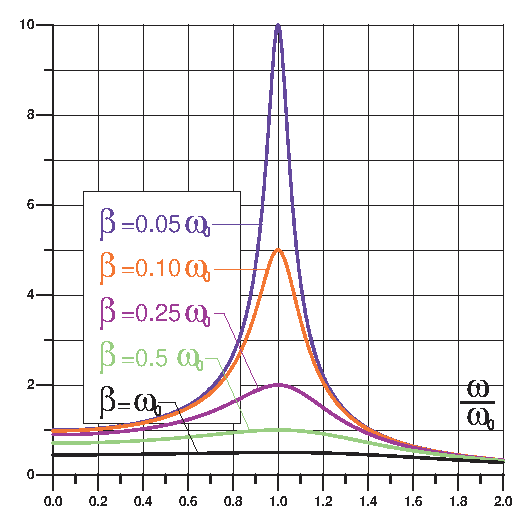
\includegraphics{GP014F32.eps}}
 \put(100,0){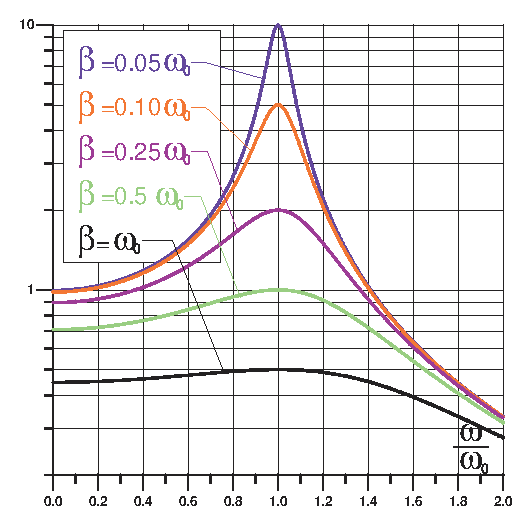
\includegraphics{GP014F33.eps}}
 \put(0,33){\makebox(0,0)[tl]{\parbox{165mm}{
 }}}
\end{picture}\\
Если бы сопротивление полностью отсутствовало (чего в действительности, конечно не бывает), то резонанс наступил бы при $\omega=\omega_0$, и амплитуда выросла бы до $\infty$. Фаза\\
\begin{picture}(185,60)(0,0)
 %\put(0,0){\framebox(185,65)[b]{}}
 \put(70,0){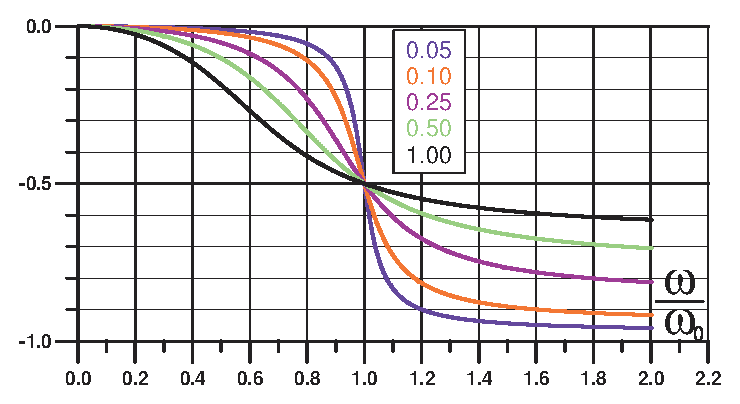
\includegraphics{GP014F34.eps}}
 \put(0,57){\makebox(0,0)[tl]{\parbox{65mm}{
 колебания отстает при ре\-зонансе от фазы вы\-ну\-ж\-да\-ю\-щей силы ровно на $\frac\pi 2$; получается, что сила каждый раз подталкивает систему по направлению ее движения, совершая положительную работу.
 }}}
\end{picture}\\[2mm]
 Эта работа никуда не тратится (трения-то нет!), а идет на неограниченное возрастание энергии системы.

 При низких частотах система просто следует за вынуждающей силой ($\alpha$=0), а при больших -- из-за своей инерционности за силой не поспевает.

 Вообще говоря, вынуждающая сила не обязательно должна меняться по гармоническому закону. Это могут быть, например, короткие импульсы. Но для достижения резонанса они должны следовать синхронно с собствен\-ной частотой колебания -- должны {\sl ``попадать в такт''}. Не обязательно каждый период, можно, например, 1 раз из 5. Пример: нужен стабильный генератор с частотой 100 МГц, а имеется кварц только на 20 МГц. Решение:\\
\begin{picture}(185,50)(0,0)
 %\put(0,0){\framebox(185,50)[b]{}}
 \put(0,0){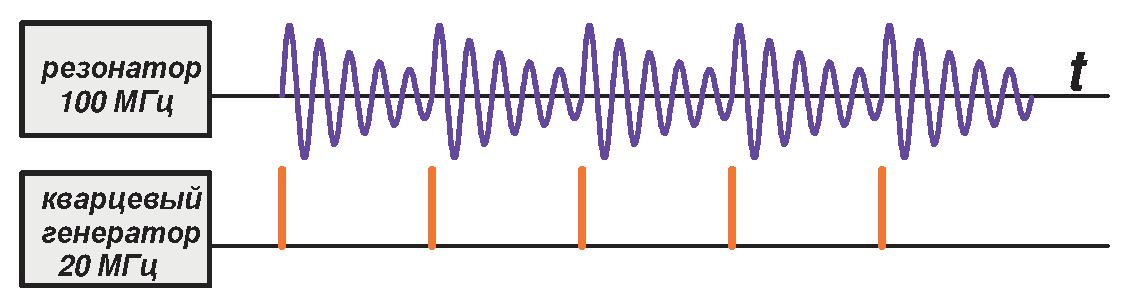
\includegraphics{GP014F36.eps}}
\end{picture}\\[2mm]

 Если синхронно меняется не сила, а параметр системы (момент инерции, длина подвеса), то это -- \underline{\bf параметрический резонанс}. Пример: человек на качелях.\\[5mm]

\centerline{\underline{\Large\bf ВОЛНЫ}}

\noindent
Если колеблющаяся точка -- в среде, все точки которой как-то связаны, то колебание может им передаваться.
Волна -- явление распространения колебаний в среде.

Частицы не перемещаются с волной, а только колеблются возле своего положения равновесия.\\
\underline{\bf Продольная волна} -- если частицы колеблются вдоль той же прямой, по которой рас\-про\-стра\-ня\-ется колебание\\
\underline{\bf Поперечная волна} -- если частицы колеблются поперек.\\
Распространение {\bf поперечной волны} возможно, если при сдвиге слоя возникают упругие возвращающие силы.\\
\begin{picture}(185,105)(0,0)
 %\put(0,0){\framebox(185,105)[b]{}}
 \put(0,0){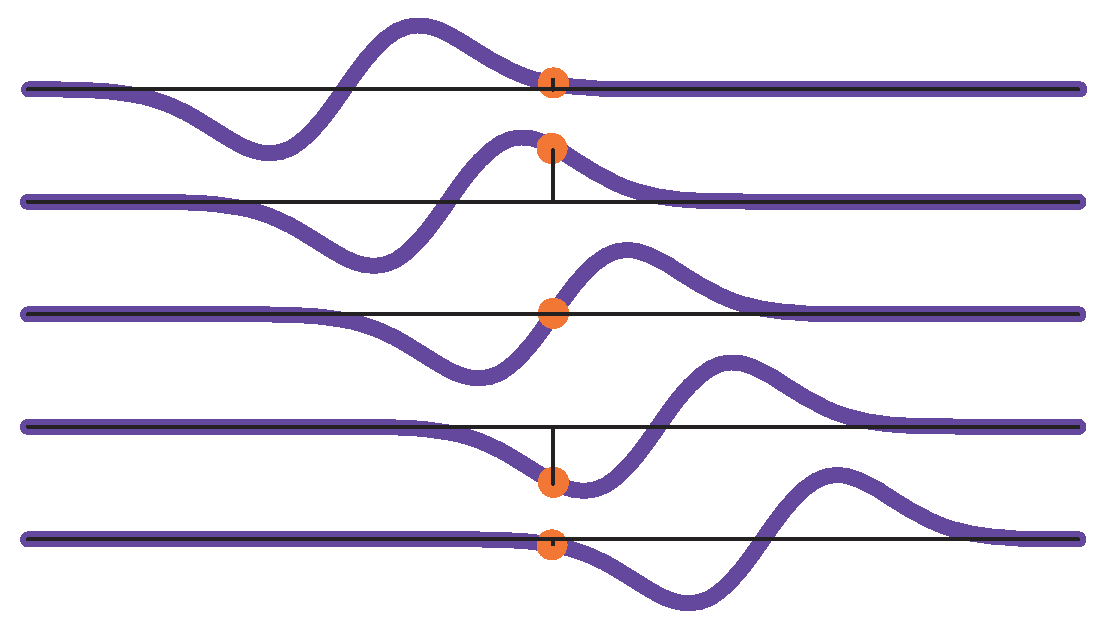
\includegraphics{GP014F37.eps}}
\end{picture}\\[2mm]

Распространение {\bf продольной волны} обусловлено повышением дав\-ле\-ния. В жидкости и газе возможны только продольные волны.\\
\begin{picture}(185,95)(0,0)
 %\put(0,0){\framebox(185,95)[b]{}}
 \put(0,0){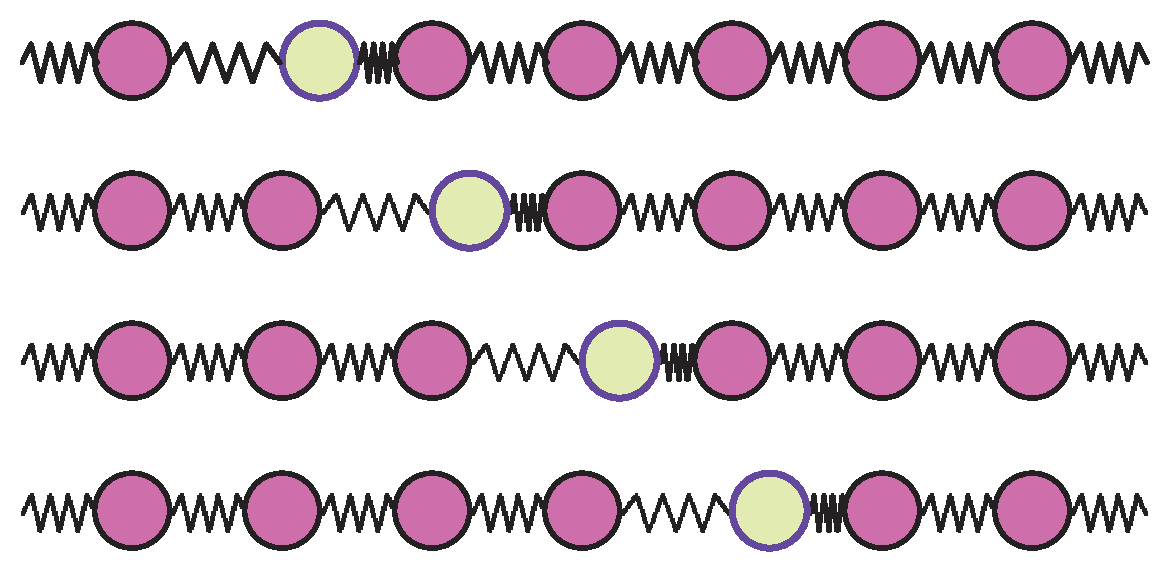
\includegraphics{GP014F38.eps}}
\end{picture}\\
\begin{picture}(185,25)(0,0)
 %\put(0,0){\framebox(185,25)[b]{}}
 \put(100,0){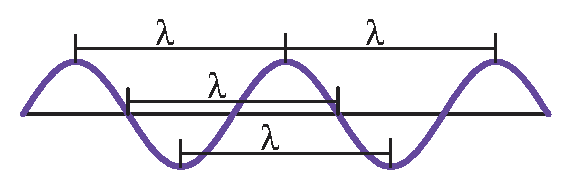
\includegraphics{GP014F39.eps}}
 \put(0,25){\makebox(0,0)[tl]{\parbox{95mm}{
 {\bf Длина волны} $\bf\lambda$ -- расстояние между ближайшими точками, колеблющимися в одинаковых фазах.
 }}}
\end{picture}\\
Скорость распространения волны $V$ -- это ее {\bf фазовая скорость}, т. е. не скорость колеблющихся точек, а скорость распространения данной фазы колебания.\\
Направления распространения колебаний -- {\bf лучи}.\\
Г.м.т., до которых к некоторому моменту дошло колебание -- {\bf фронт волны}.\\
Г.м.т., колеблющихся в одинаковых фазах, -- {\bf волновая поверхность}. (Фронт волны -- частный случай волновой поверхности). В изотропной среде колебания от центра колебаний тоже распространяются изотропно, и волновые поверхности -- сферы, а лучи направлены по радиусам.\\
Форма фронта $\Rightarrow$ тип волны (плоская, цилиндрическая, и т. п.).\\
\begin{picture}(185,70)(0,0)
 %\put(0,0){\framebox(185,70)[b]{}}
 \put(0,0){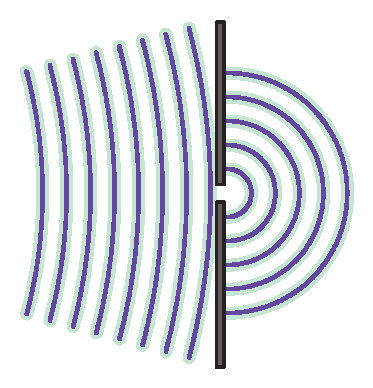
\includegraphics{GP014F40.eps}}
 \put(125,0){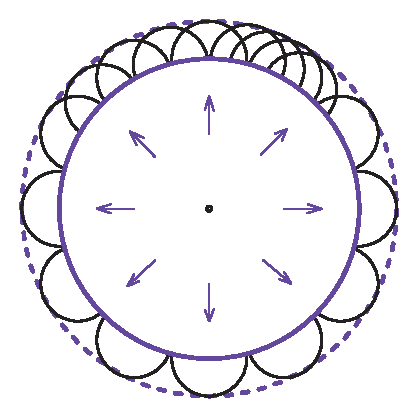
\includegraphics{GP014F41.eps}}
 \put(40,67){\makebox(0,0)[tl]{\parbox{98mm}{
\underline{Принцип Гюйгенса (1629--1695, Гаага)}
метод построения волнового фронта
 }}}
 \put(60,50){\makebox(0,0)[tl]{\parbox{62mm}{
Каждая точка су\-ще\-с\-т\-ву\-ю\-ще\-го волнового фрон\-та рас\-сма\-т\-ри\-ва\-ет\-ся как ис\-то\-ч\-ник но\-во\-го ко\-ле\-ба\-ния $\Rightarrow$ сфе\-ри\-че\-с\-кие вол\-ны $\Rightarrow$ оги\-ба\-ю\-щая = новый фронт.
 }}}
\end{picture}\\[2mm]
  В изотропной среде у сферической волны фронт -- это сфера. При $R\rightarrow\infty$ фронт -- это плоская волна.\\
\begin{picture}(185,55)(0,0)
 %\put(0,0){\framebox(185,55)[b]{}}
 \put(0,0){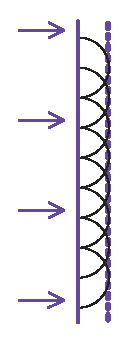
\includegraphics{GP014F42.eps}}
 \put(140,0){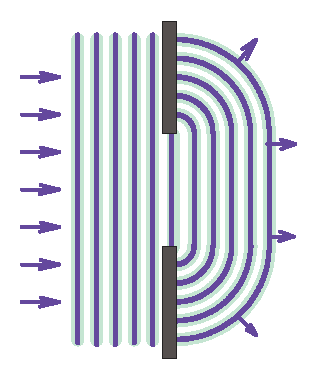
\includegraphics{GP014F43.eps}}
 \put(20,47){\makebox(0,0)[tl]{\parbox{118mm}{
 Если на пути волны оказывается препятствие с отверстием $>\lambda$, то центральная часть волны пройдет прямо, а по краям направление изменится -- явление \underline{\bf диффракции}. Чем меньше размеры отверстия -- тем сильнее выражена диффракция.
 }}}
\end{picture}\\
\underline{\bf Уравнение волны}\\
\begin{picture}(185,40)(0,0)
 %\put(0,0){\framebox(185,35)[b]{}}
 \put(0,0){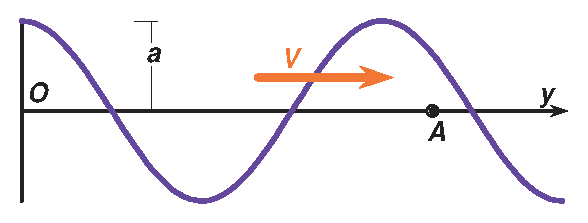
\includegraphics{GP014F44.eps}}
 \put(100,44){\makebox(0,0)[tl]{\parbox{90mm}{
 Пусть из точки $O$ в направлении $y$ со скоростью $V$ распространяется волна. Колебания в точке $O$:\\
  $x=a\,\cos(\omega t)$. До произвольной точки $A$ на рас\-сто\-я\-нии $y$ волна докатится за время $\tau=y/V$.
 }}}
\end{picture}\\
Таким образом, точка $A$ тоже начнет колебаться с такой же частотой и амплитудой, но с запаздыванием на время $\tau$:
\begin{displaymath}
x=a\,\cos\omega(t-\tau)=a\,\cos\omega\left(t-\frac yV\right)=
a\,\cos\left(\omega t-2\pi\frac y\lambda\right)
\end{displaymath}
 Если расстояние между точками = целому числу волн $(n\cdot\lambda)$, то они колеблются в одинаковой фазе, а если полуцелому $(n\cdot\lambda+\frac\lambda2)$ -- то в противофазе.

У сферической волны ее амплитуда убывает обратно пропорционально радиусу. Поэтому ее уравнение:
\begin{displaymath}
x=\frac ar\,\cos\omega\left(t-\frac rV\right)
\end{displaymath}\\

Если есть несколько источников, то для волн соблюдается {\bf принцип суперпозиции} (волны распространяются совершенно независимо друг\\
\begin{picture}(185,80)(0,0)
 %\put(0,0){\framebox(185,80)[b]{}}
 \put(0,0){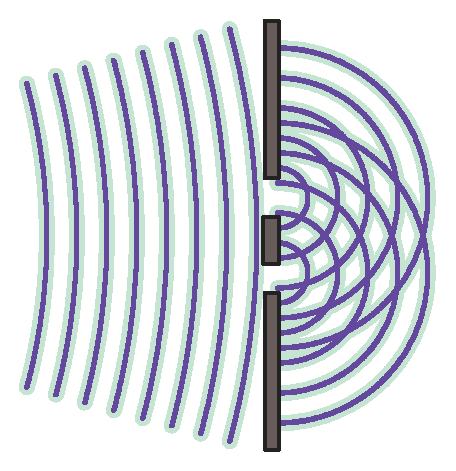
\includegraphics{GP014F45.eps}}
 \put(80,75){\makebox(0,0)[tl]{\parbox{105mm}{
 от друга, и соответствующие отклонения линейно суммируются). Если эти источники ``работают'' синхронно (с одной частотой и с постоянным сдвигом фазы), то есть, являются \underline{\bf когерентными}, то наблюдается явление \underline{\bf интерференции} волн, когда при сложении они усиливаются или, наоборот, компенсируют друг друга. }}}
\end{picture}\\

Частный случай интерференции -- когда две когерентные волны идут навстречу друг другу (чаще всего это бывает при отражении от препятствия).\\
\begin{picture}(185,60)(0,0)
 %\put(0,0){\framebox(185,50)[b]{}}
 \put(20,0){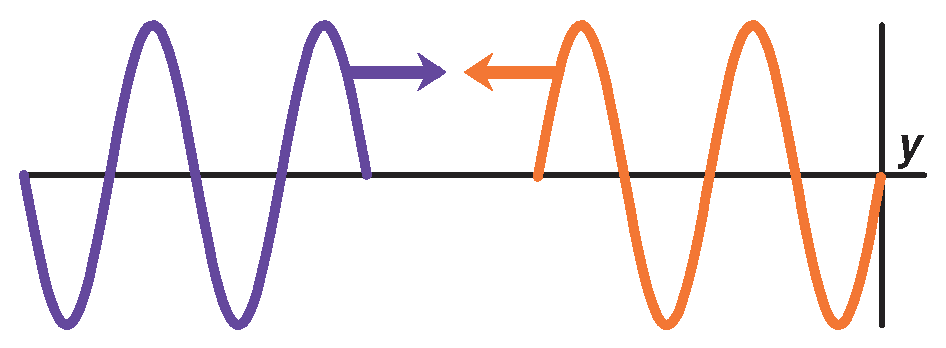
\includegraphics{GP014F46.eps}}
\end{picture}\\
Тогда колебания, вызываемые прямой и отраженной волнами, будут, со\-от\-вет\-ствен\-но:
\begin{displaymath}\begin{array}{ccc}
x_+&=&a\,\cos2\pi\left(\nu t-\frac y\lambda\right)\\
x_-&=&a\,\cos2\pi\left(\nu t+\frac y\lambda\right)
\end{array}
\end{displaymath}
Суммарное колебание по принципу суперпозиции равно
\begin{displaymath}
x=x_++x_-=a\,\cos2\pi\left(\nu t-\frac y\lambda\right)+a\,\cos2\pi\left(\nu t+\frac y\lambda\right)
\end{displaymath}
когда заменим косинус суммы, то получим:
\begin{displaymath}
x=2a\,\cos\left(2\pi\frac y\lambda\right)\cdot\cos2\pi\nu t
\end{displaymath}
Второй косинус задает колебания во времени с частотой $\nu$, а первый косинус показывает распределение амплитуды колебаний в пространстве (с периодом = длине волны $\lambda$).

Получились так называемые
\underline{\bf стоячие волны}. Они как бы не движутся вправо/влево, а колебание происходит только по вертикали (для данного примера).

Те точки в пространстве, где амплитуда максимальна, называбтся {\bf пучностями}, а где минимальна -- {\bf узлами}. Точки, симметрично рас\-по\-ло\-жен\-ные от узлов, колеблются в противофазе.

Стоячие волны бывают как поперечные, так и продольные.
\newpage
\underline{\bf Энергия волны}.\\
Пусть волна распространяется вдоль оси $y$ и описывается ур-нием
\begin{displaymath}
x=a\,\cos \omega\left(t-\frac yV\right).
\end{displaymath}
Если рассмотреть маленький участок среды объемом $\tau$, то его $E=E_k+E_p$. Посчитаем $E_k$:
\begin{displaymath}
E_k=\frac12mv^2
\end{displaymath}
учитывая, что $m=\tau\rho$, где $\rho$ -- это плотность среды, а $v=\dot{x}=\frac{dx}{dt}=-a\omega\sin \omega\left(t-\frac yV\right)$, получим:
\begin{displaymath}
E_k=\frac12\rho\tau a^2\omega^2 \sin^2 \omega\left(t-\frac yV\right).
\end{displaymath}
Если бы у нас были колебания \underline{изолированной} точки, то $E_k$ и $E_p$ все время переходили бы друг в друга, и $E_p$ вычислять было бы не обязательно. Мы бы прсто нашли МАКСИМАЛЬНУЮ $E_k$ (в этот момент $E_p$=0) и приравняли бы $E=E_k$.

Но у нас точки все связаны, и энергия переходит от одних точек к другим и обратно $\Rightarrow$ для маленького объема $\tau$ полная энергия вовсе не обязана сохраняться.

Потенциальная энергия деформированного тела (как для сжатой пру\-жи\-ны) пропорциональна жесткости $k$ и квадрату относительной деформа\-ции $\left(\frac{\Delta L}L\right)^2$. Можно показать, что относительная деформация выражается через $\frac{dx}{dy}$, а жесткость связана со скоростью распространения волны. Тогда, если все это учесть, то получится, что
потенциальная энергия маленького объема $\tau$ в точности равна кинетической и меняется с ней не в проти\-во\-фа\-зе, а в фазе! Тогда получается, что полная энергия равна
\begin{displaymath}
E=\rho\tau a^2\omega^2\sin^2\omega\left(t-\frac yV\right).
\end{displaymath}
То есть, как видим, энергия колебаний в данной точке все время меняется как $\sin^2\omega t$. Чтобы получить среднее значение, надо найти $\overline{\sin^2}$:
\begin{displaymath}
\overline{\sin^2x}=\frac{\int\limits_0^{2\pi}\sin^2x\,dx}{2\pi}=
\frac{\int\limits_0^{2\pi}(1-\cos2x)\,dx}{4\pi}=
\frac{2\pi-\int\limits_0^{2\pi}\cos2x\,dx}{4\pi}=\frac12
\end{displaymath}
Плотность энергии волны в данной точке -- это энергия на единицу объема:
\begin{displaymath}
\varepsilon=\frac E\tau=\frac12\rho a^2\omega^2.
\end{displaymath}
Поскольку волна движется со скоростью $V$, то она переносит энергию от точки к точке.\\
\begin{picture}(185,50)(0,0)
 %\put(0,0){\framebox(185,50)[b]{}}
 \put(0,0){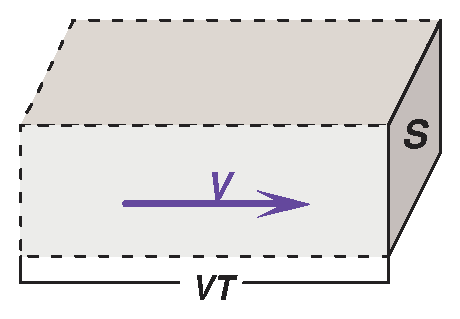
\includegraphics{GP014F47.eps}}
 \put(80,53){\makebox(0,0)[tl]{\parbox{105mm}{
 Через площадку $S$ за время $T$ проносится энергия $E$, содежащаяся в столбе длиной $VT$:  $E=\varepsilon\,VTS$. Введем понятия потока энергии $P$ и его плотности $U$:\vspace{-4mm}
 \begin{displaymath}
 \vec{P}=\frac{E}{T}=\varepsilon \vec{V}S;\;\;\;\; \vec{U}=\frac{P}{S}=\varepsilon \vec{V}
 \end{displaymath}
 Оба они -- векторы (как и $\vec{V}$), причем $\vec{U}$
 }}}
\end{picture}\\
называют вектором Умова-Пойнтинга.

 Пусть источник волны -- точечный, тогда сферическая волна будет нести энергию по радиусам. Если поток энергии $P$ через всю сферу не зависит от того, ГДЕ мы проведем эту сферу, то его плотность $U$ -- зависит:
 \begin{displaymath}
 U=\frac{P}{S}=\frac{P}{4\pi R^2}.
 \end{displaymath}
 Важный вывод: плотность потока энергии от точечного источника падает с расстоянием как $\frac1{R^2}$.\\

 \underline{\bf Эффект Доплера }. (Christian Doppler, 1803--1853, Зальцбург, Прага, Вена)\\
 Что будет, если источник и приемник волн движутся относительно друг друга в среде, где волны распространяются со скоростью $V$? Будем считать, что скорость источника $u>0$ если он приближается к приемнику. Точно так же будем считать, что скорость приемника $v>0$ если он приближается к источнику.
 \begin{itemize}
 \item $v=u=0$. Приемник примет столько волн, сколько мимо него пройдет, а пройдет -- столько, сколько испустит источник. Т.е., $\nu_{\rm receiver} =\nu_{\rm source}$ (как и ожидалось).
 \item Источник неподвижен ($u=0$), а приемник движется ($v\neq0$).\\
  \begin{picture}(185,55)(0,0)
  %\put(0,0){\framebox(185,55)[b]{}}
  \put(0,0){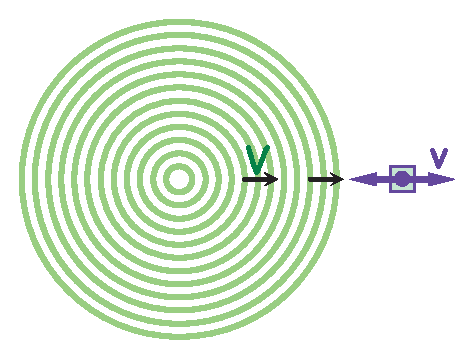
\includegraphics{GP014F48.eps}}
  \put(80,52){\makebox(0,0)[tl]{\parbox{95mm}{
  Приемник при движении навстречу волнам будет натыкаться на них чаще, чем если бы он был неподвижен. Расстояние между волнами по-прежнему = $\lambda$, но вместо скорости $V$ надо брать встречную скорость $V+v$, и тогда регистрируемая частота будет  }}}
  \end{picture}\\
 выше при движении навстречу и ниже при движении прочь от источника:
 \begin{displaymath}
  \nu_r=\frac{V+v}{\lambda}=\nu_s\left(1+\frac{v}{V}\right)
 \end{displaymath}
 \item Приемник неподвижен ($v=0$), а источник движется ($u\neq0$).\\
  \begin{picture}(185,55)(0,0)
  %\put(0,0){\framebox(185,55)[b]{}}
  \put(-5,0){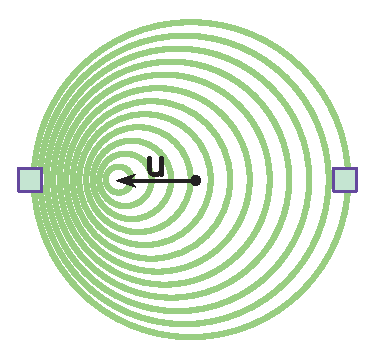
\includegraphics{GP014F49.eps}}
  \put(110,0){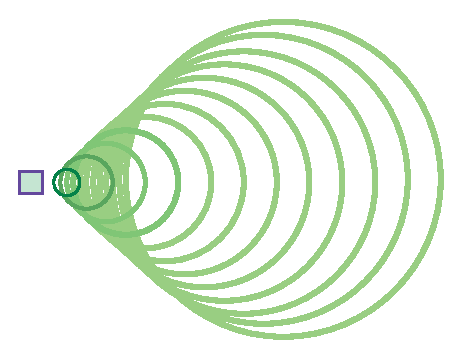
\includegraphics{GP014F50.eps}}
  \put(58,52){\makebox(0,0)[tl]{\parbox{48mm}{
  Каждая новая вол\-на излучается из но\-вого места, и их карта в про\-странстве ан\-и\-зо\-троп\-на. Если источник прибли-
  }}}
  \end{picture}\\
 жается к приемнику ($u>0$), то расстояние между волнами $<\lambda$, и они регистрируются чаще, а если удаляется ($u<0$), то волны регистрируются реже:
 \begin{displaymath}
  \lambda^\prime=\lambda-uT=VT-uT=(V-u)T;
 \end{displaymath}
 \begin{displaymath}
  \nu_r=\frac{V}{\lambda^\prime}=\frac{V}{(V-u)T}=\nu_s\,\frac{V}{V-u}
 \end{displaymath}
 \item И приемник, и источник движутся. В этом случае оба явления имеют место, и регистрируемая частота определяется как
 \begin{displaymath}
  \nu_r=\frac{V+v}{\lambda^\prime}=\frac{V+v}{(V-u)T}=\nu_s\,\frac{V+v}{V-u}
 \end{displaymath}
 \end{itemize}
Если скорости $u$ и/или $v$ превосходят скорость распространения волн $V$, то возможны всякие забавные ситуации (баллистическая волна при пролете сверхзвукового самолета).

Что если скорость $V$ очень большая (=с)?  В этом случае сложение скоростей происходит не линейно, а по совсем другому закону. Встречная скорость источника и приемника $v'$ вычисляется по релятивистской формуле:
\begin{displaymath}
v'=\frac{v-u}{1-\frac{vu}{c^2}},
\end{displaymath}
а скорость волн =$с$ во всех системах отсчета. Поэтому и эффект Доплера записывается иначе:
\begin{displaymath}
 \nu_r=\nu_s\,\left(1+\frac {v'}c\right)
\end{displaymath}
Как вы должны помнить, именно на этой разнице и основывался эксперимент Майкельсона-Морли.

Здесь уже важна только взаимная встречная скорость $v'$. Если источник и наблюдатель сближаются, то  $\exists$ фиолетовое смещение, а если удаляются -- то красное.

Применение: астрофизика (результат астрономических наблюдений -- расширяющаяся Вселенная); эффект Мессбауэра (прецизионные из\-ме\-ре\-ния скоростей); радиолокация (селекция движущихся целей); ГИБДД.\\

\underline{\bf Акустические колебания (звук).}
Человеческое ухо сполобно ре\-а\-ги\-ро\-вать на звук в диапазоне от 20 до 20,000 Гц (Heinrich Rudolf Hertz, 1857--1894, Карлсруэ, Берлин, Бонн). Инфразвук (<20 Hz) и ультразвук (>20 kHz).

Скорость звука зависит от плотности и упругости среды. Можно по\-ка\-зать, что для газов скорость звука
\begin{displaymath}
V=\sqrt{\frac{\gamma RT}{\mu}}\;\;\;\;\;\texttt{где}\;\;\;\gamma=\frac{C_p}{C_V}=\frac{i+2}i
\end{displaymath}
-- не зависит от давления, но $\propto$ корню из температуры. При н.у. скорость звука в разных газах: воздух -- 331 м/с, водород -- 1284 м/с.

В воде $V$=1485 м/с, в твердых телах -- от 2 до 6 км/с.
\end{document}
